\documentclass[10pt]{article}

\usepackage{fancyhdr}
\usepackage[includeheadfoot,left=1in, right=0.5in, top=0.5in, bottom=0.5in]{geometry}
\usepackage{lastpage}
\usepackage{extramarks}
\usepackage[usenames,dvipsnames]{color}
\usepackage{graphicx}
\usepackage{listings}
\usepackage{courier}
\usepackage{tikz}
\usepackage{color}
\usepackage{float}
\usepackage{url}
\usepackage{subfigure}
\usepackage{varwidth}
\usepackage{caption}
\usepackage{multirow}
\usepackage[pdfborder={0 0 0}]{hyperref}
\usepackage[compact,small]{titlesec}
\usepackage{microtype}
\usepackage{verbatim}
\usepackage{booktabs}
\usepackage{indentfirst}
\usepackage{pbox}
\usepackage{dcolumn}
\usepackage{pgffor}

\parskip = 0.5\baselineskip
\setlength{\belowcaptionskip}{-\baselineskip}

\captionsetup{font=scriptsize}
\captionsetup{labelfont=bf}

\pagestyle{fancy}
\rhead{Max Thrun | Samir Silbak}
\lhead{EECE6086 - HW 2}
\rfoot{Page\ \thepage\ of \protect\pageref{LastPage}}
\cfoot{}
\renewcommand\headrulewidth{0.4pt}
\renewcommand\footrulewidth{0.4pt}

% make verbatim text small
\makeatletter
\g@addto@macro\@verbatim\tiny
\makeatother

\setlength\parindent{0pt} % Removes all indentation from paragraphs

\definecolor{sh_comment}{rgb}{0.12, 0.38, 0.18 } %adjusted, in Eclipse: {0.25, 0.42, 0.30 } = #3F6A4D
\definecolor{sh_keyword}{rgb}{0.37, 0.08, 0.25}  % #5F1441
\definecolor{sh_string}{rgb}{0.06, 0.10, 0.98} % #101AF9

\lstset{
    language=c++,
    xleftmargin=.25in,
    xrightmargin=.25in,
    numbers=left,
    numberstyle=\tiny,
    frame=tb,
    showstringspaces=false,
    captionpos=b,
    stringstyle=\color{sh_string},
    keywordstyle = \color{sh_keyword}\bfseries,
    commentstyle=\color{sh_comment}\itshape,
    basicstyle=\footnotesize\sffamily,
    %numbersep=-5pt,
    belowskip=\baselineskip,
    aboveskip=\baselineskip
}

\let\oldtabular\tabular
\renewcommand{\tabular}{\footnotesize\oldtabular}

\newcommand{\placementimage}[2]{
    \begin{figure}[H]
        \centering
        \includegraphics[width=\linewidth, height=4in, keepaspectratio]{#1}
        \caption{#2}
    \end{figure}
}

\newcommand{\specialcell}[2][c]{\textbf{\begin{tabular}[#1]{@{}c@{}}#2\end{tabular}}}

\title{
    \vspace{2in}
    \textmd{\textbf{EECE6086 - HW 2}}\\
    \vspace{4in}
}
\author{\textbf{Max Thrun | Samir Silbak}}

\begin{document}
\maketitle
\newpage
\section{Objective}

\section{Implementation Details}

\subsection{Placement}

    \subsubsection{Placement Grid Dimensions}

        One of the main goals of this project is to have a final layout that is
        as close to a perfect square as possible. We call this the
        \texttt{squareness} of our layout which is the ratio of width to height
        \texttt{squareness = width / height}.  The closer this value is to 1
        the `more square' the layout is.  The main issue with achieving this is
        that we do not know up front how tall our layout will end up since the
        channels between the cells are variable and the width and hight of the grid
        directly effect them.

        In order to figure out what width and height we should make our grid we need
        to come up with some heuristic that can estimate the squareness of a layout
        given only the placement grid dimensions, number of cell, and number of nets.

        \begin{figure}[H]
            \centering
            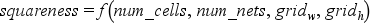
\includegraphics{./square_f.png}
            \caption{Squareness Function}
        \end{figure}

        Once we have an equation that can estimate the squareness we can plug
        in different grid dimensions and figure out one that gets us the best
        squareness. In order to figure out the formula that estimates our
        squareness we manually specified various grid dimensions for each
        benchmark and recorded the resulting squareness. This data can be found
        in the Appendix section at the end of the report. We then used the
        program Eureqa to evolve an equation that fit our data. After running
        Eureka for 15 minutes we had an equation that fit our data with an $
        R^{2} =  0.9965 $.

        \begin{figure}[H]
            \centering
            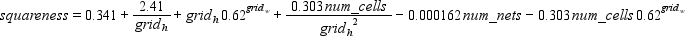
\includegraphics[width=\linewidth]{./square_eq.png}
            \caption{Squareness Equation}
        \end{figure}

        To calculate the placement grid size we start the grid as a perfect
        square by taking the square root of the number of cells. We then
        decrease the height and increase the width and check the squareness of
        this size. We continue doing this and keeping track of which size
        results in the best squareness until the height is 0.

        The table below shows the resulting squareness of the original method
        (just making a perfectly square grid) versus using the equation. We
        can see that by using the equation we achieved a much more square
        layout for all but benchmark 9. This could be a result of not having
        enough data points to fit a better curve with.

        \begin{table}[H]
            \centering
            \begin{tabular}{c|ccc|ccc|c}
                \toprule
                & \multicolumn{3}{c}{\specialcell{Without Equation}} & \multicolumn{3}{|c|}{\specialcell{With Equation}} & \\
                \textbf{Benchmark} &
                \specialcell{Grid\\Width} & \specialcell{Grid\\Height} & \specialcell{Squareness} &
                \specialcell{Grid\\Width} & \specialcell{Grid\\Height} & \specialcell{Squareness} &
                \specialcell{Percent\\Improvement} \\
                \midrule
                 1  & \phantom{0}7 & \phantom{0}7 & 0.7245 & \phantom{0}9 & \phantom{0}5 & 1.0789 &           19.66 \% \\
                 2  &           10 & \phantom{0}9 & 0.7365 &           12 & \phantom{0}8 & 0.9845 &           24.80 \% \\
                 3  &           14 &           13 & 0.6767 &           18 &           10 & 1.0914 &           23.18 \% \\
                 4  &           19 &           19 & 0.7029 &           28 &           13 & 1.2579 & \phantom{0}3.92 \% \\
                 5  &           27 &           27 & 0.6125 &           45 &           16 & 1.2060 &           18.16 \% \\
                 6  &           32 &           32 & 0.6060 &           56 &           18 & 1.1735 &           22.05 \% \\
                 7  &           23 &           22 & 0.6452 &           39 &           13 & 0.9823 &           33.71 \% \\
                 8  &           30 &           30 & 0.6306 &           50 &           18 & 1.3123 & \phantom{0}5.70 \% \\
                 9  &           29 &           28 & 0.6343 &           45 &           18 & 1.4323 &           -6.67 \% \\
                 10 &           25 &           24 & 0.6715 &           36 &           17 & 1.2772 & \phantom{0}5.13 \% \\
                \bottomrule
            \end{tabular}
            \caption{Improvement from using squareness estimate equation}
        \end{table}

        \newpage
        \subsubsection{Force Directed Placement}

        We use a force directed placement algorithm in order to reduce the
        overall complexity. Our algorithm follows the one in the book exactly
        with the exception of what happens when the target cell is locked.  In
        the original algorithm you search for a vacant spot to place the seed
        cell, we expand that to also include unlocked spots. If we choose an
        unlocked spot the that cell we are replacing becomes the new seed cell.
        We found though experiementation that this achieves less complex
        placements.

        \begin{figure}[H]
            \centering
            \includegraphics[width=\linewidth, height=2in, keepaspectratio]{../benchmarks/10_placement_0_start.jpg}
            \caption{Original}
        \end{figure}
        \begin{figure}[H]
            \centering
            \includegraphics[width=\linewidth, height=2in, keepaspectratio]{../benchmarks/10_placement_1_force.jpg}
            \caption{Force Directed}
        \end{figure}

        In order to figure out the best abort limit we recorded the layout area
        for each benchmark for various limits. We found the abort limit that
        achived the minimum area and used that minimum area to normalize the
        areas of the others as a percent increase. We found that an abort limit
        of 1 gives us the lowest average percent increase in area across all
        the benchmarks.

        \begin{figure}[H]
            \centering
            \begin{minipage}{.5\textwidth}
                \centering
                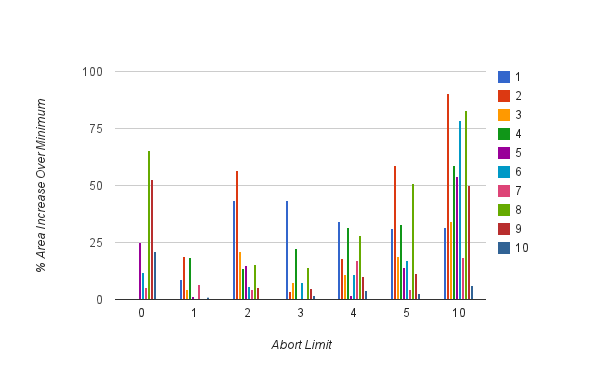
\includegraphics[width=0.98\linewidth]{./abort_limit.png}
            \end{minipage}%
            \begin{minipage}{.5\textwidth}
                \centering
                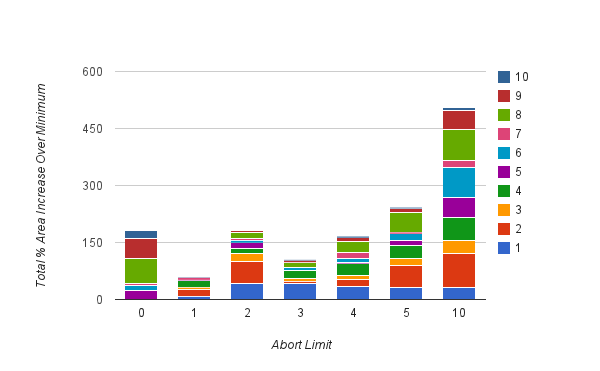
\includegraphics[width=0.98\linewidth]{./abort_limit_stacked.png}
            \end{minipage}
            \caption{Percent increase in layout area versus abort limit}
        \end{figure}

        \subsubsection{Flipping Cells}

        The force directed algorithm does not take into account the positions
        of the terminals on each cell, it assumes all connections go to the
        center of the cell. This results in a lot of connections that
        unnecessarily span vertically across a row. To fix these we simply go
        through each cell and try all possible flip orientations and see which
        one reduces the wirelength the most. This approach is not ideal as it
        does not take into consideration chains of cells that all may need to
        be flipped. An approach similar to KL where we walk down the connection
        tree trying flips and only actually flipping as many as what improves
        the total wirelength would be interesting. Unfortunately we did not
        have time to explore this.

        \begin{figure}[H]
            \centering
            \includegraphics[width=\linewidth, height=4in, keepaspectratio]{../benchmarks/10_placement_1_force.jpg}
            \caption{Original}
        \end{figure}
        \begin{figure}[H]
            \centering
            \includegraphics[width=\linewidth, height=4in, keepaspectratio]{../benchmarks/10_placement_2_flip.jpg}
            \caption{Flipped}
        \end{figure}

        \subsubsection{Adding Feed Throughs}

        \subsubsection{Evening Row Lengths}

        \subsubsection{Pulling Cells Closer}

        \subsubsection{Moving Feed Throughs}


\subsection{Routing}

\newpage
\section{Usage}


\newpage
\section{Results}

\foreach \i in {1,...,10} {
    \newpage
    \subsection{Benchmark \i\thinspace - Placement Steps}
    \placementimage{../benchmarks/\i_placement_0_start.jpg}      {Benchmark \i\thinspace - Step 1/7 - Initial placement}
    \placementimage{../benchmarks/\i_placement_1_force.jpg}      {Benchmark \i\thinspace - Step 2/7 - Force directed placement}
    \placementimage{../benchmarks/\i_placement_2_flip.jpg}       {Benchmark \i\thinspace - Step 3/7 - Flip cells}
    \placementimage{../benchmarks/\i_placement_3_feed.jpg}       {Benchmark \i\thinspace - Step 4/7 - Add feed throughs}
    \placementimage{../benchmarks/\i_placement_4_feed_even.jpg}  {Benchmark \i\thinspace - Step 5/7 - Even out the row length}
    \placementimage{../benchmarks/\i_placement_5_pull.jpg}       {Benchmark \i\thinspace - Step 6/7 - Pull cells in the rows closer together}
    \placementimage{../benchmarks/\i_placement_6_feed_moved.jpg} {Benchmark \i\thinspace - Step 7/7 - Move feed throughs to optimal location}

    \newpage
    \subsection{Benchmark \i\thinspace - Final Routing}
    \begin{figure}[H]
        \centering
        \includegraphics[width=\linewidth, height=4.5in, keepaspectratio]{../benchmarks/\i.jpg}
        \caption{Benchmark \i\thinspace - Final routing}
    \end{figure}

    %\newpage
    %\subsection{Benchmark \i\thinspace - Log}
    \lstinputlisting[caption=Benchmark \i\thinspace - Log]{../benchmarks/\i.log}
}

\newpage
\section{Performance Trends}

\newpage
\section{Appendix}

\begin{table}[H]
    \centering
    \begin{tabular}{cccccc}
        \toprule
        \textbf{Benchmark} & \textbf{Num Cells} & \textbf{Num Nets} & \textbf{Grid Width} & \textbf{Grid Height} & \textbf{Squareness}\\
        \midrule

        1  & 45   & 45   & 7  & 7  & 0.72449 \\
        2  & 90   & 90   & 10 & 9  & 0.736486 \\
        3  & 180  & 180  & 14 & 13 & 0.676724 \\
        4  & 360  & 360  & 19 & 19 & 0.702857 \\
        5  & 720  & 720  & 27 & 27 & 0.612457 \\
        6  & 1000 & 1000 & 32 & 32 & 0.605988 \\
        7  & 500  & 1000 & 23 & 22 & 0.645203 \\
        8  & 900  & 720  & 30 & 30 & 0.630648 \\
        9  & 800  & 360  & 29 & 28 & 0.634349 \\
        10 & 600  & 180  & 25 & 24 & 0.67148 \\
           &      &      &    &    & \\
        1  & 45   & 45   & 8  & 6  & 0.820225 \\
        2  & 90   & 90   & 27 & 8  & 0.984496 \\
        3  & 180  & 180  & 12 & 12 & 0.755981 \\
        4  & 360  & 360  & 15 & 18 & 0.740413 \\
        5  & 720  & 720  & 20 & 26 & 0.595577 \\
        6  & 1000 & 1000 & 28 & 31 & 0.561298 \\
        7  & 500  & 1000 & 33 & 21 & 0.614935 \\
        8  & 900  & 720  & 24 & 29 & 0.637652 \\
        9  & 800  & 360  & 32 & 27 & 0.685294 \\
        10 & 600  & 180  & 30 & 23 & 0.75 \\
           &      &      &    &    & \\
        1  & 45   & 45   & 9  & 5  & 1.078947 \\
        2  & 90   & 90   & 13 & 7  & 1.20339 \\
        3  & 180  & 180  & 17 & 11 & 0.921875 \\
        4  & 360  & 360  & 22 & 17 & 0.833333 \\
        5  & 720  & 720  & 29 & 25 & 0.681979 \\
        6  & 1000 & 1000 & 34 & 30 & 0.583232 \\
        7  & 500  & 1000 & 25 & 20 & 0.646465 \\
        8  & 900  & 720  & 33 & 28 & 0.672032 \\
        9  & 800  & 360  & 31 & 26 & 0.731629 \\
        10 & 600  & 180  & 28 & 22 & 0.773946 \\
           &      &      &    &    & \\
        1  & 45   & 45   & 12 & 4  & 1.779661 \\
        2  & 90   & 90   & 15 & 6  & 1.623762 \\
        3  & 180  & 180  & 18 & 10 & 1.091429 \\
        4  & 360  & 360  & 23 & 16 & 0.84127 \\
        5  & 720  & 720  & 30 & 24 & 0.742911 \\
        6  & 1000 & 1000 & 35 & 29 & 0.624372 \\
        7  & 500  & 1000 & 27 & 19 & 0.692828 \\
        8  & 900  & 720  & 34 & 27 & 0.711864 \\
        9  & 800  & 360  & 32 & 25 & 0.790323 \\
        10 & 600  & 180  & 29 & 21 & 0.869748 \\
           &      &      &    &    & \\
        1  & 45   & 45   & 15 & 3  & 2.923077 \\
        2  & 90   & 90   & 18 & 5  & 1.864583 \\
        3  & 180  & 180  & 20 & 9  & 1.322368 \\
        4  & 360  & 360  & 24 & 15 & 0.920382 \\
        5  & 720  & 720  & 32 & 23 & 0.75098 \\
        6  & 1000 & 1000 & 36 & 28 & 0.699068 \\
        7  & 500  & 1000 & 28 & 18 & 0.715323 \\
        8  & 900  & 720  & 35 & 26 & 0.694501 \\
        9  & 800  & 360  & 34 & 24 & 0.810289 \\
        10 & 600  & 180  & 30 & 20 & 0.991111 \\
           &      &      &    &    & \\
        1  & 45   & 45   & 23 & 2  & 4.945946 \\
        2  & 90   & 90   & 23 & 4  & 2.626667 \\
        3  & 180  & 180  & 23 & 8  & 1.391608 \\
        4  & 360  & 360  & 26 & 14 & 0.986532 \\
        5  & 720  & 720  & 33 & 22 & 0.848671 \\
        6  & 1000 & 1000 & 38 & 27 & 0.674667 \\
        7  & 500  & 1000 & 30 & 17 & 0.763196 \\
        8  & 900  & 720  & 36 & 25 & 0.832599 \\
        9  & 800  & 360  & 35 & 23 & 0.883333 \\
        10 & 600  & 180  & 32 & 19 & 1.074074 \\

        \bottomrule
    \end{tabular}
    \caption{Squareness Trial Data}
\end{table}


\end{document}
